% ===========================================================================
%  N4a.9 --- the sliding ratio, read three ways.
%
%  Section 5.4 states in one sentence that the endpoint 1/a is where the next
%  three sections live.  This draws that sentence: one clock, one endpoint,
%  three operations on it, three laws out.
%
%  Build:  latexmk -pdf figure.tex   (writes ../../N4a_9_three_readings.pdf)
% ===========================================================================
\documentclass[11pt,tikz,border=4pt]{standalone}

\usepackage[T1]{fontenc}
\usepackage{lmodern}
\usepackage{amsmath,amssymb}
\usepackage{tikz}
\usetikzlibrary{arrows.meta,positioning,calc}
% ===========================================================================
%  tikz_style.tex --- shared TikZ styles for this chapter's schematic figures.
%
%  The upstream style file named by the older figure sources no longer exists
%  on this machine; this replaces it, matching the palette of style_rc.py so
%  that the TikZ schematics and the matplotlib plots read as one set.
%      bdc ink        #1a1c1f      bdc soft   #565b62
%      bdc blue       #0072B2      bdc grid   #e3e6ea
% ===========================================================================

\definecolor{bdcink}{HTML}{1A1C1F}
\definecolor{bdcsoft}{HTML}{565B62}
\definecolor{bdcblue}{HTML}{0072B2}
\definecolor{bdcgrid}{HTML}{E3E6EA}

\tikzset{
  % axes and event arrows
  bdc arrow/.style={
    draw=bdcink, line width=0.5pt,
    -{Stealth[length=4.5pt,width=3.2pt]},
  },
  % the absorbing rupture state
  bdc catastrophe/.style={
    draw=bdcink, line width=0.6pt, circle, fill=bdcgrid,
    inner sep=1.6pt, minimum size=13pt,
    font=\small,
  },
  % marginal commentary, deliberately quieter than the diagram
  bdc annotation/.style={
    text=bdcsoft, font=\small\itshape,
  },
  % rate and level labels sitting against the path
  bdc ratelabel/.style={
    text=bdcink, font=\small,
  },
}


\tikzset{
  reading/.style={
    draw=bdcgrid, line width=0.7pt, rounded corners=1pt,
    text=bdcink, align=left, inner sep=5pt,
    minimum height=15mm, text width=44mm,
  },
  fan/.style={draw=bdcsoft, line width=0.5pt,
              -{Stealth[length=4pt,width=2.8pt]}},
  verb/.style={text=bdcsoft, font=\small, inner sep=1.5pt},
}

\begin{document}
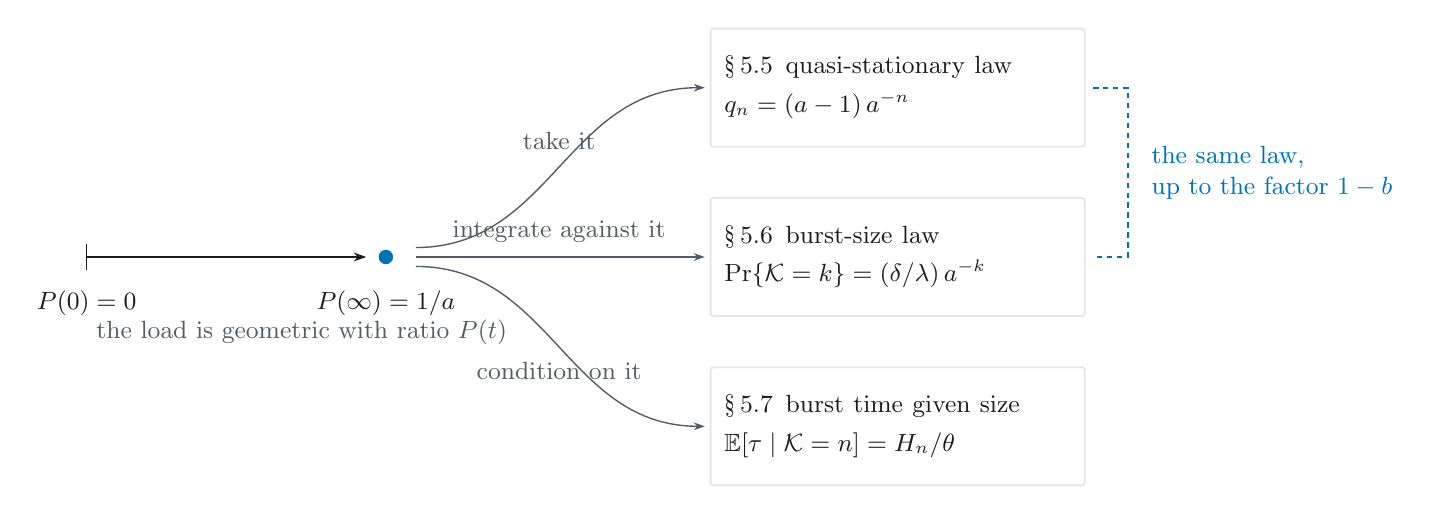
\begin{tikzpicture}[x=1cm,y=1cm]

  % ---- the clock -----------------------------------------------------------
  \draw[bdc arrow] (0,0) -- (3.55,0);
  \draw[draw=bdcink,line width=0.5pt] (0,-0.16) -- (0,0.16);
  \node[font=\small,text=bdcink,anchor=north] at (0,-0.3) {$P(0)=0$};
  \fill[bdcblue] (3.8,0) circle (2.6pt);
  \node[font=\small,text=bdcink,anchor=north] at (3.8,-0.3) {$P(\infty)=1/a$};
  \node[font=\small,text=bdcsoft,anchor=west] at (0,-0.95)
    {the load is geometric with ratio $P(t)$};

  % ---- three readings of that one endpoint ---------------------------------
  \node[reading] (qsd)   at (10.3, 2.15)
    {\small \S\,5.5\enspace quasi-stationary law\\[2pt]
     $q_n=(a-1)\,a^{-n}$};
  \node[reading] (burst) at (10.3, 0.00)
    {\small \S\,5.6\enspace burst-size law\\[2pt]
     $\Pr\{\mathcal K=k\}=(\delta/\lambda)\,a^{-k}$};
  \node[reading] (time)  at (10.3,-2.15)
    {\small \S\,5.7\enspace burst time given size\\[2pt]
     $\mathbb E[\tau\mid\mathcal K=n]=H_n/\theta$};

  \draw[fan] (4.18,0.12) .. controls (5.9,0.12) and (6.1,2.15) .. (7.85,2.15);
  \draw[fan] (4.18,0.00) -- (7.85,0.00);
  \draw[fan] (4.18,-0.12) .. controls (5.9,-0.12) and (6.1,-2.15) .. (7.85,-2.15);

  \node[verb,anchor=south] at (6.0, 1.30) {take it};
  \node[verb,anchor=south] at (6.0, 0.12) {integrate against it};
  \node[verb,anchor=north] at (6.0,-1.28) {condition on it};

  % ---- and two of the three are the same law -------------------------------
  \draw[draw=bdcblue,line width=0.7pt,dash pattern=on 2pt off 1.6pt]
    (12.78,2.15) -- (13.22,2.15) -- (13.22,0.00) -- (12.78,0.00);
  \node[text=bdcblue,font=\small,anchor=west,align=left] at (13.4,1.07)
    {the same law,\\up to the factor $1-b$};

\end{tikzpicture}
\end{document}
